\chapter{Control, Simulation, and Visualization Software}
\label{ch:software}

\section{Visualizer}

The Eelume Visualizer refers to software developed as part of this thesis to 
visualize the pose of the Eelume robot in real time during experimental 
operations. The necessity for such a tool became apparent during initial 
testing on the Eelume robot. The default software suite used for Eelume 
provides a map view of the robot's position and displays Euler angles, position,
and joint angles as numerical values on a screen. This setup makes it 
difficult to gain a quick and intuitive understanding of the robot's current 
configuration, particularly in observing how it evolves over time. The Eelume 
Visualizer addresses this issue by presenting a real-time computer-generated 
rendering of the robot.

% features
The visualizer offers a wide range of features. The rendering of the Eelume 
robot is based on 3D object files supplied by Eelume AS, which enhances the 
realism of the visualization. Joints can be configured to arbitrary angles, 
and their motion is accurately represented through the bending of the 
connected links. The visualizer includes a grid in the north-east plane and 
displays an \gls{ned} axis at the coordinate origin, providing spatial context 
and aiding in visualizing depth and orientation. Additionally, it supports 
rendering spheres of arbitrary color and position, which has been extensively 
used to depict desired task values. This allows users to intuitively assess 
how effectively a controller is executing a task without needing to analyze 
numerical data.

The visualizer supports switching between different fields of view and 
projection methods, including both perspective and orthographic projections. 
When appropriately positioned, the camera also enables an isometric view. 
These capabilities make the visualizer well-suited for professional 
presentation of specific Eelume configurations. In fact, all computer-
generated imagery of the Eelume robot presented in this thesis was created 
using the visualizer. It includes built-in screenshot functionality, allowing 
for the export of images with a transparent background (\(0\) alpha value). An 
optional shadow projection feature enhances spatial perception by casting a 
shadow onto the virtual ground plane.

% how it was made
The visualizer is implemented in pure C++ using OpenGL in conjunction with the 
GLEW and GLFW libraries. All shaders, which manage scene lighting, are written 
in the OpenGL shading language \textit{GLSL} and were developed as part of 
this thesis. This includes custom shading for the joints, which required 
specialized mathematical treatment to bend accurately. These joint shaders 
were implemented using the matrix exponential of \(\se\) elements, as 
described mathematically in \autoref{ch:appendix:math}.

% how it works (udp)
The robot's position, along with the color and position of the spheres, is 
controlled externally through messages sent via \gls{udp}. This allows for 
straightforward integration and control from virtually any programming language
. A lightweight C++ header file was created to expose functions for setting 
the robot's pose and rendering spheres.

An example of the visualizer in use during an experiment is shown in
\autoref{fig:eelume:visualizer}. The background grid lines and the central
axis system illustrate the origin of the \gls{ned} frame.
\begin{figure}[h!]
    \centering
    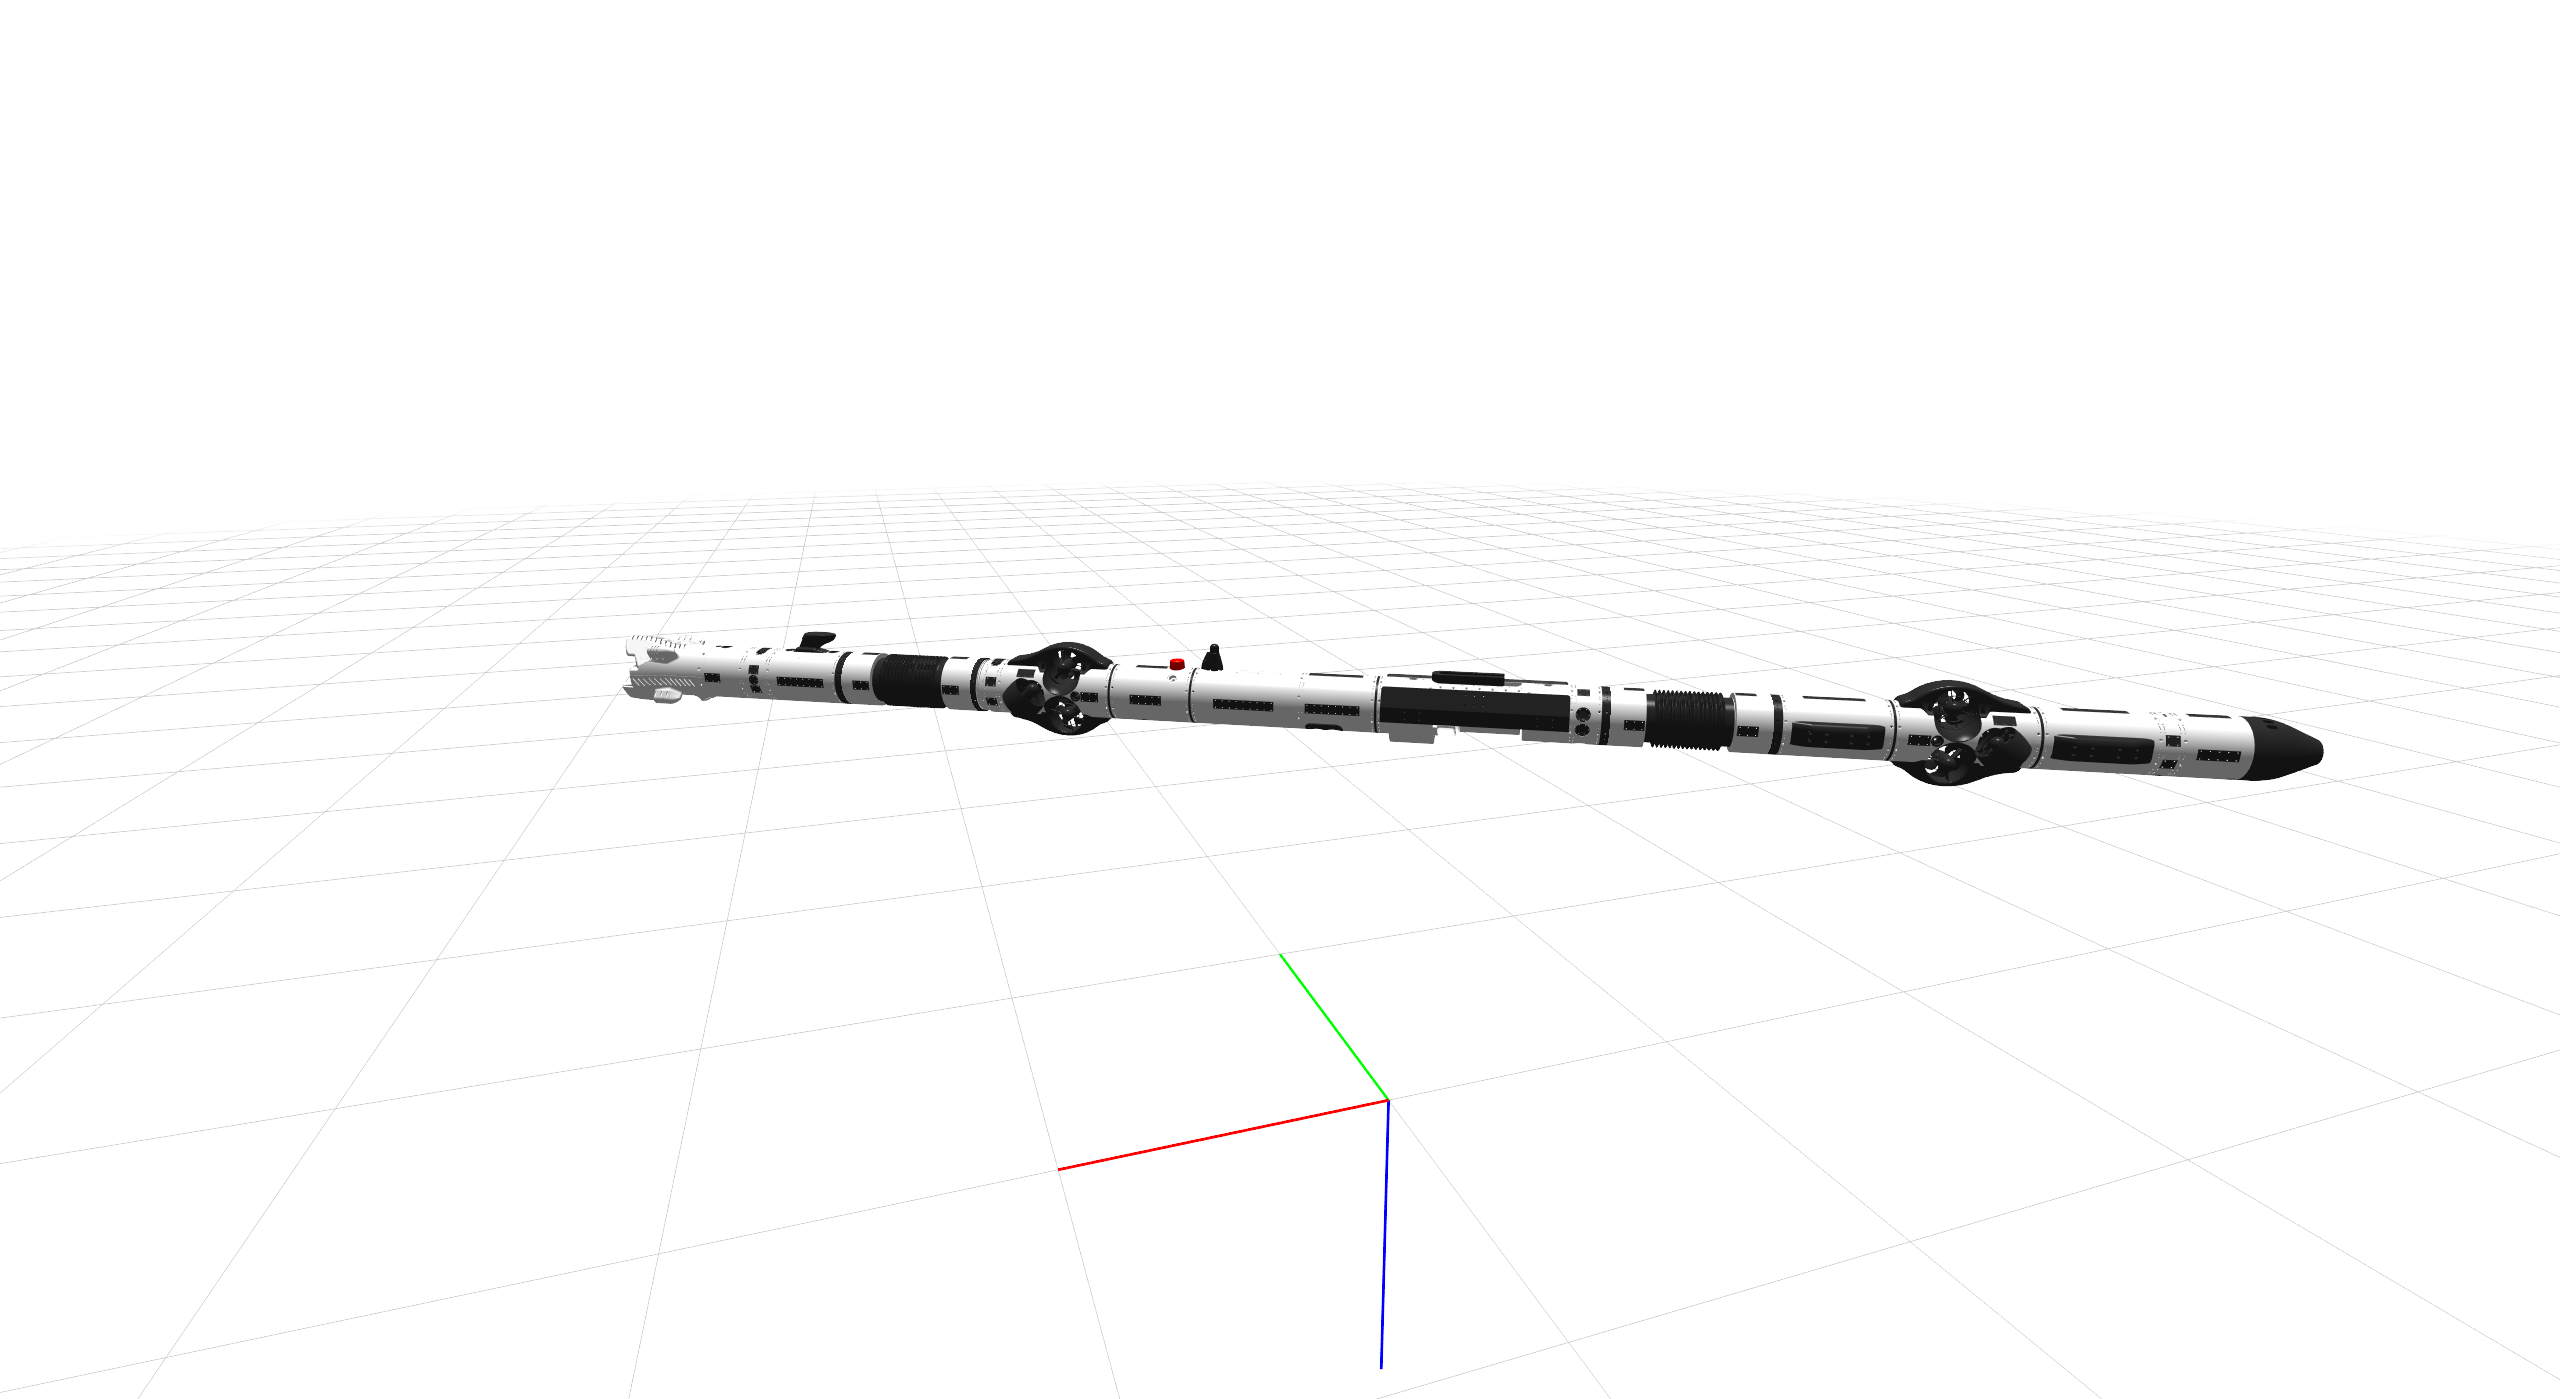
\includegraphics[width=\textwidth]{assets/eely-visualizer.png}
    \caption{A screenshot of the Eelume visualizer.}
    \label{fig:eelume:visualizer}
\end{figure}

\FloatBarrier

\section{EelyControlKit}

\iffalse
\gls{eck} referrs to a C++ library made as part of this thesis for controlling the Eelume robot.
To better
understand how this library works and why it is needed, some background information
about the internals of the Eelume robot is needed.

The Eelume robot is controlled using a low-level \gls{api} made available by Eelume AS
in the beginning of 2025. This \gls{api} provides access to an internal \gls{can} bus, which is used to
communicate with the robot's thrusters, joints, and sensors. The \gls{api} can
be used to write arbitrary messages on this bus, but also has a set functions
for sending predefined messages which different components of the robot will
send and receive. For instance, when setting thruster force- and joint
torque-references, several messages has to be sent on this bus for the
thrusters to set their internal references.

The \gls{api} is implemented in C/C++ and communicates with the robot over
an ethernet connection. Because the \gls{api} is low-level, a lot of code had
to be written to implement the \gls{tpc} framework, everything from
lower-level controllers, mathematics, task definitions, kinematics and dynamics.
The collection of code build on top of this low-level \gls{api} is referred to as \gls{eck}.

A design decision was made to build this control kit as a library, the vision
is to allow for easy development of arbitrary controllers, not only task-priority
controllers, and give the tools and mathematics needed to do such a thing. The library
is build in C++, partially because the lower-level api is in C/C++, and partially because
of the computational requirements of task-priority controllers. Development in
C++ allows for fast runtimes at the cost of compile time. \Gls{eck} being built
as a library means it can be compiled once and then linked to for faster compile
times and good abstractions.

% -----------------------------------------------------------------------------
\subsection{Features}

% connection to the Eelume robot
Among the primariy features of the \gls{eck} is a connection class representing
open communication between the actual Eelume robot and software. This class takes
care of all the neccessary setup, subscribing to incomming messages, parsing of data,
and sending data in the correct format. The class expose a \textit{connect} function
and returns an object returning a representation of the connection if successfull. 
Throughtut the codebase, \textit{optionals}, a C++ 17 feature, to elegantly handle
unexpected errors and invalid states. As part of this connection class, functions
for setting references for thrusters and joint motors are also implementd, allowing
for fast testing without having to re-write code.

% kinematics and jacobians and (B) matrix
An other important contribution is the kinematics class. This class represent
the kinematics of the Eelume robot and gives access to important methods based
on kinematics. The class translates and returns transformations between frames,
as well as calculating jacobians. This calss is extensively used when calculating
the task jacobians used in the task-priority controllers. Using the kinematics
along with some specification of the thruster configuration allows for the caluculation
of the thruster allocation matrix \(\bm{B}\) in \autoref{eq:modeling:Bdef}. Allowing
for thruster allocation by a simple pseudo-inverse.

% a set of controllers
Among the fetures of the \gls{eck} is a set of pre defined controllers. This indcludes a
simple \gls{pd}-controller, \gls{pd+} controller, and velocity-level task-priority controllers.
All the controllers are implemented using a common interface, allowing for switching
of controller on runtime, rateher than compile-time, if that is desireable. The implemented
task-priority controller is general in the sense that it allowes for arbitrary null-space
projector method, with the standard successive and augmented being implemented. A \textit{task}
class is also implemented, automatically computing task jacobians for position and
orientation tasks based on the given kinematics.

% mathematical and utility functions
A set of mathematical and utility functions are also implemented. This includes
simple mathematical functions, like rotation matrices, skew products, and similar.
It also includes more complex functions, like a Runge-Kutta integrator taking
an arbitrary lambda function, and a reference generator using the Runge-Kutta integrator
to low-pass filter a reference and output desired task values as well as their
derivatives for use in control.
\fi

\gls{eck} refers to a C++ library developed as part of this thesis for controlling the Eelume robot.  
To better understand the purpose and functionality of this library, some background information on the internal workings of the Eelume robot is necessary.

The Eelume robot is controlled using a low-level \gls{api} provided by Eelume AS in early 2025. This \gls{api} grants access to the internal \gls{can} bus, which is used for communication with the robot's thrusters, joints, and sensors. While the \gls{api} allows for sending arbitrary messages over this bus, it also includes a set of functions for transmitting predefined messages used by various robot components. For example, setting thrust and joint torque references requires sending multiple messages across the bus for the thrusters to correctly adjust their internal references.

The \gls{api} is implemented in C/C++ and communicates with the robot via an Ethernet connection. Due to its low-level nature, significant additional code was required to implement the \gls{tpc} framework, including modules for lower-level controllers, mathematical operations, task definitions, and kinematic and dynamic modeling. This codebase, built atop the low-level \gls{api}, is referred to as \gls{eck}.

A key design decision was to develop this control kit as a reusable library. The goal is to facilitate the development of a wide range of controllers, not only task-priority controllers, by providing the necessary tools and mathematical infrastructure. The library is written in C++, partly to align with the low-level API and partly due to the computational demands of task-priority control. Using C++ ensures fast runtimes, albeit at the cost of longer compile times. Since \gls{eck} is built as a library, it can be compiled once and linked for subsequent use, enabling faster compilation and maintaining clean abstractions.

% -----------------------------------------------------------------------------
\subsection{Features}

% connection to the Eelume robot
One of the primary features of \gls{eck} is a connection class that encapsulates the communication between the Eelume robot and external software. This class handles all necessary setup, message subscriptions, data parsing, and formatting for transmission. It exposes a \textit{connect} function that returns an object representing the connection if successful. Throughout the codebase, C++17 \textit{optionals} are used to elegantly manage unexpected errors and invalid states. Additionally, the connection class provides functions for setting references for thrusters and joint motors, enabling quick testing without rewriting code.

% kinematics and jacobians and (B) matrix
Another major contribution is the kinematics class. This class represents the robot’s kinematic model and provides access to a range of methods rooted in kinematics. It computes and returns transformations between frames and calculates Jacobians. It is extensively used in computing task Jacobians for task-priority control. Combined with a specification of the thruster configuration, the kinematics class enables computation of the thruster allocation matrix \(\bm{B}\) in \autoref{eq:modeling:Bdef}, which is then used for simple pseudo-inverse-based thruster allocation.

% a set of controllers
Among the features of \gls{eck} is a collection of pre-defined controllers. This includes a simple \gls{pd} controller, a \gls{pd+} controller, and velocity-level task-priority controllers. All controllers adhere to a common interface, which allows switching between controllers at runtime instead of compile time, if desired. The implemented task-priority controller is general and supports arbitrary null-space projection methods, with standard successive and augmented methods included. A \textit{task} class is also provided, which automatically computes task Jacobians for position and orientation tasks using the given kinematic model.

% mathematical and utility functions
A suite of mathematical and utility functions is also included. These range from basic operations, such as rotation matrices and skew-symmetric products, to more advanced tools like a Runge-Kutta integrator that accepts arbitrary lambda functions. A reference generator is also implemented using this integrator, which allows for low-pass filtering of references and outputs desired task values along with their derivatives for use in control algorithms.

% -----------------------------------------------------------------------------
\section{Simulator}

As part of \gls{eck} a built in simulator was implemented. 
The simulator is designed to mimic the behavior of the Eelume robot as closely
as possible, 
without much time spent on modeling the hydrodynamics and coupling
between the links.
The kinematics of the robot is thought to be accurately
implemented. Because of the virtual base classes, the real robot can be used
interchangeably without recompiling the code. This allows for easy testing of
the controllers after verifying that they work in the simulator.

\begin{itemize}
    \item 
\end{itemize}


\begin{itemize}
    \item Connection to EelyControlKit
\end{itemize}

\section{Conclusion}

The simulator

The visulalizer

EelyControlKit

